\documentclass[11pt]{article}

\usepackage[margin=1in]{geometry}
\usepackage{mathptmx}
\usepackage[T1]{fontenc}
\usepackage[utf8]{inputenc}
\usepackage{microtype}
\usepackage{graphicx}
\usepackage{booktabs}
\usepackage{amsmath}
\usepackage{amssymb}
\usepackage{array}
\usepackage{ragged2e}
\usepackage{caption}
\usepackage{xcolor}
\usepackage[numbers,sort&compress]{natbib}
\usepackage[colorlinks=true,linkcolor=blue!45!black,citecolor=blue!45!black,urlcolor=blue!45!black]{hyperref}

\captionsetup{font=small,labelfont=bf}
\graphicspath{{figures/}}
\newcommand{\code}[1]{\texttt{#1}}

\title{\bfseries From Self-Reports to Track Records:\\ Calibration-Robust Task Allocation for Decentralised Multi-Agent LLM Systems}
\author{Teo Qing Cong Eugene\\ \small Independent \\ \small \texttt{redacted}}
\date{\today\\[2pt] \small\itshape Plain-language edition. A technical edition with identical results and figures is available as \texttt{main\_formal.tex}.}

\begin{document}
\maketitle

\begin{abstract}
\noindent
Many multi-agent systems are run by one central orchestrator that hands out work from the top. This puts two costs on a single node: it must judge every candidate for every task, and its own speed limits the whole system. We study an alternative, Chemotactic Task Allocation (CTA), a decentralised design inspired by biology and with no central assigner. Each task advertises a short description of what it needs (a semantic envelope). Each agent scores how well it matches, and volunteers only when that match clears a set threshold, the activation barrier. Among the volunteers, the winner has the highest Binding Energy: a score that rewards a good match and a strong track record and divides by cost. Before the winner may write anything, an integrity gate checks that it is reliable and in scope. This design leans on one assumption: that an agent can judge its own fit. That is exactly where language-model agents are known to be unreliable, so we do not assume the self-rating is correct; we treat it as a variable and vary it on purpose. Across three settings, a pre-registered protocol on synthetic populations, a fleet tuned to measured model calibration, and a live pilot with real coding agents, we find the same story. Miscalibration (an agent misjudging itself) is the main way self-selection fails, and a simple correction wins back most of the loss: discount each self-rating by the agent's observable track record, which needs no privileged information. The gate then guards against agents that try to game the system. On scaling, the decentralised design keeps peak per-node load flat (fitted growth exponent $0.0$), while a central scheduler grows as $N\times M$ (exponent $2.0$) out to ten thousand agents, a roughly $250\times$ saving in coordinator cost at representative prices. We are careful about the quality claim: against a full-information optimum, which no real deployment could build, CTA does not clear its pre-registered margin, and we report that honestly; against the information-bounded central scheduler a deployment would actually run, decentralised self-selection matches it when information is fresh and pulls ahead as the central reliability table goes stale. Finally, on real Claude agents across three model families, the same two ideas become a cost result. A task wrapper (an explicit interface contract) lifts a weak model to a frontier model's completion, and it is what lets modules built by different agents fit into one working project. A calibrated agent wrapper then routes each task to the cheapest capable model, holding frontier-level completion at roughly one fortieth of the always-frontier cost, but only when the tasks are wrapped, so the two wrappers are complementary. Every result is deterministic and reproduced from seeds by one command, and the real-agent results are powered (about ten agents per cell for the ladder, five for the project) with bootstrap confidence intervals.
\end{abstract}

\section{Introduction}

Multi-agent systems increasingly coordinate large numbers of autonomous agents across many tasks at once. A common design puts one central orchestrator in charge of handing out the work from the top down. This is easy to reason about, but it piles two costs onto a single node. The coordinator has to judge candidates for every task, and its own throughput caps the throughput of the whole system. As the number of agents and tasks grows, that central node becomes a bottleneck and a single point of failure.

Decentralised alternatives have a long history. The Contract Net Protocol \citep{smith1980contractnet} spreads control through an announce, bid, and award exchange, though the award for each task still passes through a manager. Market and auction-based allocation, surveyed by \citet{dias2006market} and formalised by \citet{gerkey2004taxonomy}, treats allocation as an optimisation problem and shows where decentralised methods trade optimality for scalability. Stigmergic methods such as ant colony optimisation \citep{dorigo1996ant} coordinate indirectly, through signals left in a shared environment, with no central assigner at all. Together these show that decentralised allocation works. But three gaps recur. The award step is often still centralised for each task. A trust or reliability check before execution is rarely built in. And there is seldom a principled account of tasks that simply cannot be done with the agents available.

We study a decentralised framework, Chemotactic Task Allocation (CTA), that closes those three gaps. Its selection principle comes from two places in biology. From cryptic female choice it borrows the idea that selection continues after the first encounter, biased by chemical signals rather than settled by a single authority \citep{fitzpatrick2020cryptic}. From the response-threshold model of division of labour in social insects it borrows the activation barrier: an individual takes on a task only when the task's stimulus passes its personal threshold \citep{bonabeau1996threshold}. In computing terms, each task carries a wrapper (the scent envelope) that reads an agent's role, skills, and prompt against what the task needs, and turns that into a compatibility score $c\in[0,1]$. Agents then self-select. An agent may take a task only when its compatibility reaches the task's activation energy ($c\geq E_a$). Among the agents willing to take it, the winner is the one with the highest Binding Energy, $B=c\cdot\tilde{C}/L$: a score that rewards a good match and a strong record and divides by cost. Selection runs in two stages, a yes/no eligibility filter and then the activation barrier, followed by a separate trust stage, the Rejection Gate. We use the biology as design intuition, not as a literal specification.

It helps to compare CTA with a simple pull-based work queue, where agents just take the best task available. CTA adds three things on top: the activation barrier as a quality floor, the Rejection Gate as a trust boundary, and the eligibility filter with its notions of infeasible and stalled tasks. Our evaluation includes a pull-based baseline (Section~\ref{sec:baseline}) to isolate these additions, so a result is not merely the effect of going decentralised.

Any design in which agents choose their own tasks rests on one load-bearing assumption: that an agent can judge its own fit for a task. Recent studies of auctions and bidding among large language model agents find that their self-reported success rates are systematically off, so an allocation built from self-reports drifts away from the full-information optimum \citep{fradkin2026marketbench}, and fixing that self-confidence is still an open problem \citep{zhang2026confidence}. So we treat self-assessment as a first-class variable and vary it deliberately, rather than assuming it is right. In our model the compatibility score is the agent's self-report, drawn from its true fit plus a bias and some noise, while the quality it actually delivers depends on its true fit and real competence. Miscalibration therefore corrupts the allocation without touching the ground truth. Two questions follow. First, how badly does miscalibration hurt a self-selection allocation? Second, can an observable track record (the reliability $R$), which needs no privileged information, win the loss back? The Rejection Gate then acts as a safety backstop. This shifts the contribution away from decentralised self-selection, which is by now well covered, and onto the calibration robustness of self-selection, which is not.

Cost-aware model selection is an active area. LLM cascades and learned routers send easy queries to a cheap model and hard ones to a strong model, cutting inference cost several-fold with little quality loss \citep{chen2023frugalgpt,ong2024routellm}. CTA's agent wrapper is a router in this family, but it differs on three points. First, it corrects the routing signal for miscalibration: the bid is the model's own self-report, discounted by an observable track record, rather than a fixed capability estimate or a preference-trained classifier, so it stays honest even when a model is wrong about itself, which \citet{fradkin2026marketbench} shows is common. Second, it routes decomposed work: together with the task wrapper's interface contract, it assembles a single project from modules built by different models, which whole-query routers do not do. Third, it runs on a decentralised substrate whose coordination cost stays flat as the fleet grows. A direct head-to-head against these routers on a shared benchmark is the natural next step, and we mark it as such.

\paragraph{Contributions.}
\begin{enumerate}\itemsep2pt
\item A decentralised allocation framework in which tasks advertise semantic envelopes and agents self-select by affinity, reducing per-task coordination to an atomic claim rather than a central assignment.
\item A two-stage selection model that separates categorical capability (eligibility) from graded affinity (activation energy), and yields a principled distinction between infeasible tasks (no eligible agent) and stalled tasks (eligible agents present, none clearing $E_a$).
\item A reliability and integrity trust gate that screens degraded and out-of-scope agents before they gain write access, evaluated as a safety backstop against adversarial agents.
\item An evaluation methodology comparing the framework against centralised baselines on scaling and match quality, including an information-bounded central scheduler as the fair, beatable comparison the full-information optimum cannot provide, and a token/dollar cost model that turns coordinator work into money.
\item A study of self-assessment miscalibration as the failure mode of self-selection: the compatibility bid is treated as the agent's self-report, and a track-record correction (the reliability $R$), which uses no privileged information, recovers the completion that miscalibration costs, with the integrity gate as a safety backstop.
\item External validity in three steps: a mixed fleet whose calibration archetypes are parameterised from measured LLM behaviour (MarketBench); a live pilot with real Claude coding agents; and a capability ladder across three real model families (Haiku 4.5, Sonnet 5, Opus 4.8) that measures what the task wrapper and agent wrapper buy.
\item A self-improvement result that reads the loop as a harness \citep{weng2026harness}: a persistent, accumulating track record makes the allocation improve from its own experience toward the full-information optimum with no privileged information, while a memoryless baseline stays flat.
\end{enumerate}

\paragraph{Scope and non-goals.} This is a simulation study with real-agent confirmation, not a live deployment. The atomic claim assumes a single logical coordination store providing compare-and-swap, so the framework reduces central work rather than removing it entirely. The security model covers reliability scoring and scope integrity, and extends to two forms of gaming (bid inflation and reputation sandbagging), addressed in Section~\ref{sec:results}; cross-agent collusion is left as future work.

\section{Methodology}

\subsection{Research design}
This is a comparative, controlled experiment. We measure two systems on the same task and agent populations: the decentralised framework and a centralised baseline. Both systems share the same scoring function (Binding Energy), so the only thing that differs is how allocation is coordinated. We vary the population size to test the scaling hypothesis, and we run each configuration over many seeded replications so we can report intervals rather than single numbers. We use two modes. A simulation mode runs many synthetic agents in Python, which gives scale, determinism, and cheap sweeps. A real-swarm pilot uses Claude Code subagents competing over a shared store (SQLite), where the atomic claim is a genuine compare-and-swap; this gives ecological validity.

\subsection{Formal framework}
This subsection states the model precisely. The list below defines each step in order, from checking whether an agent is even allowed to take a task, through scoring and firing, to the trust gate and the feedback that updates an agent's record. There are a set of agents $A$ of size $N$ and a set of tasks $T$ of size $M$. Each task carries a scent envelope with a domain, an activation barrier $E_a$ (default $0.2$), and a priority. Each agent has a capability profile, permissions, tools, and a reliability history.

\begin{description}\itemsep2pt
\item[Eligibility (binary).] $\mathrm{elig}(a,t)=\mathbf{1}[\mathrm{ReqTool}_t\subseteq \mathrm{Tool}_a]\cdot\mathbf{1}[\mathrm{scope}_t\subseteq \mathrm{Perm}_a]$: tools and permitted scope are hard requirements. The eligible set is $A(t)=\{a: \mathrm{elig}(a,t)=1\}$; the task is \emph{infeasible} when $A(t)$ is empty.
\item[Compatibility and reliability.] Compatibility $c(a,t)\in[0,1]$ is produced by the task wrapper from the agent's role, skills, and prompt against the task requirements. Reliability $R(a)=(s_a+1)/(n_a+2)$ is a Laplace-smoothed success ratio over a sliding window of $W$ recent attempts. Effective capability is $\tilde{C}(a,t)=C(a,t)\cdot R(a)$.
\item[Selection score.] The Binding Energy $B(a,t)=c(a,t)\cdot\tilde{C}(a,t)/\max(L(a,t),\epsilon)$, with cost $L>0$ and floor $\epsilon=0.01$, ranks the agents that have cleared activation; it does not gate firing.
\item[Activation (firing).] Activation drive $\Delta(a,t)=c(a,t)-E_{a,t}$. Firing probability $P_{\mathrm{fire}}=1$ when $\Delta\geq 0$ and $P_{\mathrm{fire}}=\exp(\Delta/T)$ when $\Delta<0$, with temperature $T\geq 0$; the deterministic threshold is the $T\to 0$ limit. The task is \emph{stalled} when $A(t)$ is non-empty and the firing set is empty.
\item[Claim and trust.] The winner is $a^*(t)=\arg\max_{a\in F(t)}B(a,t)$, committed by an atomic compare-and-swap. The Rejection Gate admits $a^*$ when $R(a^*)\geq\tau$ (default $0.6$) and the action is in scope; otherwise it deflects.
\item[Outcome and feedback.] Realised quality $Q(a,t)=\mathrm{clip}(g(S_{\mathrm{true}},C_{\mathrm{true}})+\xi)$ is a ground truth independent of the agent's self-estimate; the attempt succeeds when $Q\geq q_{\min}$, updating $(s_a,n_a)$ and hence $R$. Self-assessment acts on noisy estimates $\hat{c}=\mathrm{clip}(c+\eta)$ with $\eta\sim\mathcal{N}(b,\sigma^2)$ for bias $b$ and noise $\sigma$; activation and selection use the estimates, outcomes use the truth. Annealing relaxes $E_{a,t}\leftarrow\max(E_{a,\min},E_{a,t}-\delta)$ per waiting round.
\end{description}

We keep two costs separate. Total evaluation work is $W_{\mathrm{eval}}=\sum_t|A(t)|$ (worst case $O(NM)$): the work of judging candidates. Coordinator work is $W_{\mathrm{coord}}=\sum_t|F(t)|$: the claim attempts that actually contend at the shared store. It is the second cost, not the first, that a central node concentrates.

\subsection{Baselines}\label{sec:baseline}
The centralised baseline is a single scheduler that assigns tasks using the same scores. We use three baselines. \code{central\_best} is the full-information quality optimum for CTA's non-exclusive setting: it gives each task the agent with the highest expected realised quality (true fit $\times$ true capability), with agent reuse allowed. It is the fair upper bound CTA approaches from below, and no real deployment could build it because it needs the ground truth (reference for H2). \code{central\_bounded} is the honest scheduler a deployment would actually run: it allocates from self-reported compatibility and a reliability estimate that lags, because a central table is synchronised in batches; a staleness parameter blends the current reliability with an out-of-date value (reference for H9). The third baseline is decentralised: a pull-based work queue with no barrier and no gate, which isolates CTA's specific mechanisms from the effect of decentralisation alone.

\subsection{Analysis}
We report means with 95\% confidence intervals. For the quality and completion metrics, which are bounded and skewed, the interval is a bootstrap percentile interval rather than a normal approximation. Each headline comparison reports how many seeds per arm a power calculation ($\alpha=0.05$, power $0.8$) requires. For scaling, we fit the growth of coordinator work against $N$ in log-log space and report the exponent with a bootstrap CI. We prefer non-parametric tests (Mann-Whitney $U$) and report effect sizes alongside $p$-values. We fix the hypotheses and acceptance margins in advance, and we correct the secondary $p$-values for multiple comparisons with a Holm-Bonferroni procedure.

\subsection{Validity and threats}
The main threat is external validity: a simulation leaves out the variable latency, cost, and unpredictable output quality of live agents, and the miscalibration of an agent scoring itself. We mitigate this at two levels: a fleet whose calibration is set from the stated-versus-realised gaps MarketBench measures, and a live pilot with real Claude agents (Section~\ref{sec:results}). Reported failure rates for real multi-agent systems are high, and they are driven by specification ambiguity and coordination breakdown that a simulation does not reproduce \citep{cemri2025multiagent}. For generalisability, we re-run the pre-registered hypotheses under a second, structurally different generative family. For reproducibility, the code, seeds, and configurations are versioned, and the deterministic path reproduces exactly.

\section{Results}\label{sec:results}

One command generates these results over the full protocol (20 seeds, agent counts from 50 to 10{,}000), and we release the raw per-seed rows behind every aggregate as a flat CSV. The results tell one story. First, the decentralised design removes the coordination bottleneck (H1). Against the scheduler a deployment would actually run, it matches that scheduler and then overtakes it as the scheduler's information goes stale (H9). It pays for this with a deliberate, bounded quality cost against a full-information optimum it does not claim to beat (H2, H6). The load-bearing risk sits in self-selection itself: it rests on each agent's own self-report, and self-reports are miscalibrated. We show that this miscalibration is the failure mode (H7), that a track-record correction using no privileged information wins back what it costs (H8), and that an integrity gate is the safety backstop (H4). We then confirm the mechanism on real Claude agents and turn it into the product claim. The task wrapper raises a weak model to frontier completion (H11), and the calibrated agent wrapper delivers frontier completion at a fraction of the cost (H12). Run over many rounds, the same loop improves from its own experience (H13).

\begin{table}[t]
\centering\small
\caption{The whole study at a glance.}
\begin{tabular}{@{}p{0.20\linewidth}p{0.10\linewidth}p{0.60\linewidth}@{}}
\toprule
\textbf{Layer} & \textbf{Claim} & \textbf{Headline result} \\
\midrule
Scaling & H1 & Peak per-node load flat (exponent $0.0$) vs quadratic central ($2.0$) to 10{,}000 agents \\
Quality & H2, H6 & Reaches $\approx 94\%$ of the fair optimum; the shortfall is mostly the deliberate latency trade \\
Fair coordination & H9 & Level with a fresh central scheduler, decisively ahead ($0.88$ vs $0.64$) as its table goes stale \\
Calibration failure & H7 & Raw self-report winners over-predict success by $\approx 0.20$ (Brier/ECE $\approx 0.25$) \\
Calibration fix & H8 & Track-record correction recovers completion $0.37\to0.76$ ($p<0.001$), no privileged information \\
Safety & H4 & Integrity gate cuts out-of-scope violations by $\approx 90\%$ under adversarial agents \\
Routing/liveness & H3,H5,H10 & Barrier routes every subtask to a correct specialist ($1.00$ vs $0.25$ floor); annealing bounds stall \\
Task wrapper & H11 & Interface contract lifts the weak model $0.950\to0.986$ completion (ten agents/cell, tight CIs) \\
Agent wrapper & H12 & Calibrated routing holds frontier completion at $\approx 1/40$ of the always-frontier cost, when wrapped \\
Self-improvement & H13 & With a persistent record, completion climbs $0.36\to0.84$ over rounds toward the oracle; raw stays flat \\
\bottomrule
\end{tabular}
\end{table}

\begin{figure}[t]
\centering
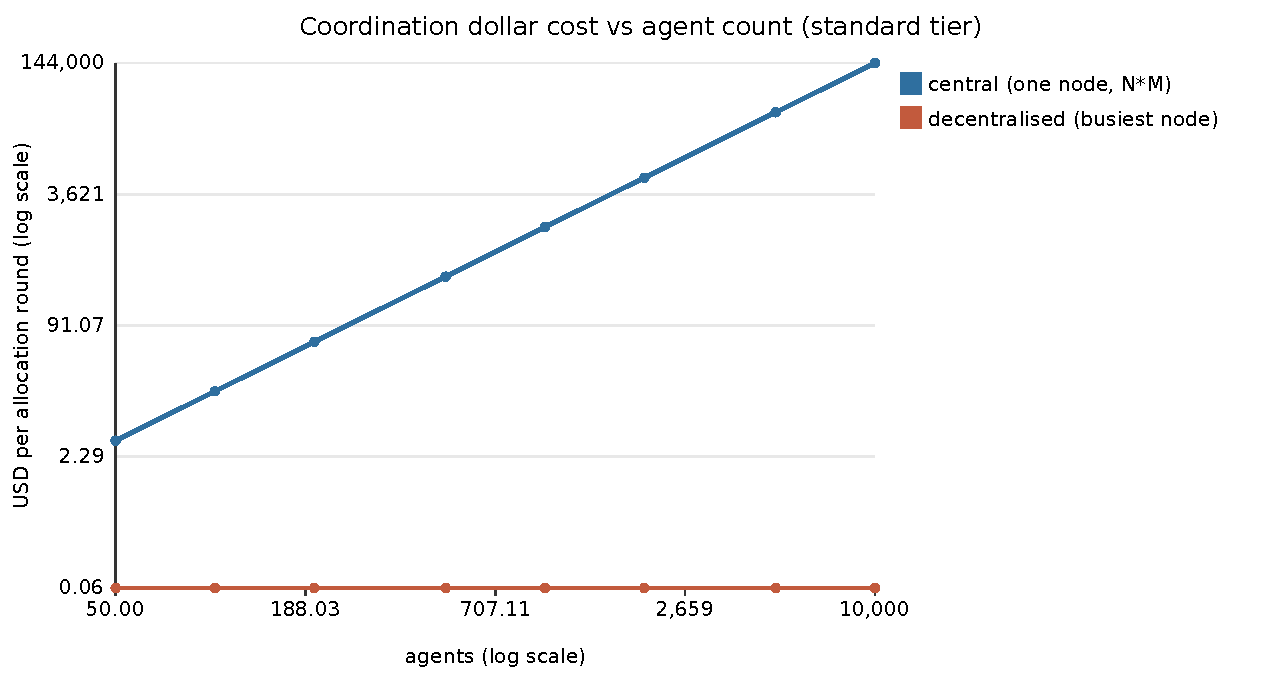
\includegraphics[width=0.86\linewidth]{cost_vs_n.pdf}
\caption{Scaling (H1). The central scheduler's coordination bill grows quadratically in fleet size while the busiest decentralised node stays flat, so the two diverge by orders of magnitude out to ten thousand agents. Prices are representative tiers.}
\end{figure}

\begin{figure}[t]
\centering
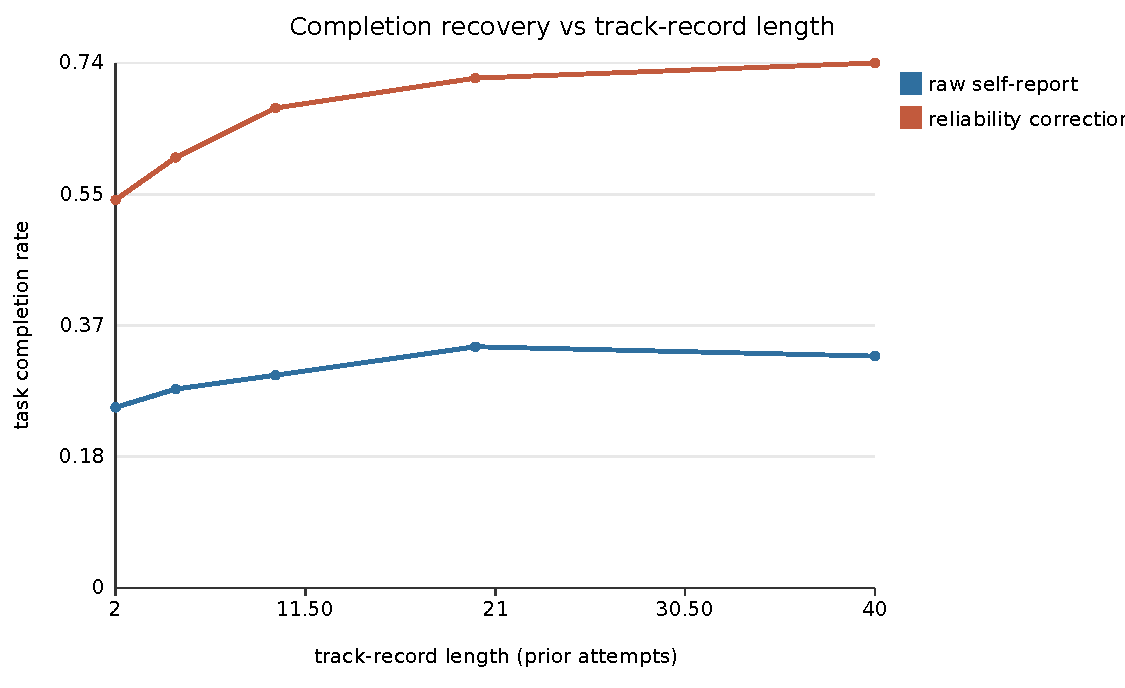
\includegraphics[width=0.78\linewidth]{track_record_recovery.pdf}
\caption{The calibration fix (H8). Discounting each self-report by the agent's observable track record recovers the completion that miscalibration costs, and the recovery needs little history: even a short record recovers most of the gap.}
\end{figure}

\subsection{Hypothesis verdicts}
Table~\ref{tab:verdicts} records the verdict for each hypothesis. Of eleven pre-registered synthetic hypotheses, nine are supported and two (the quality claims against a full-information optimum, H2 and H6) are reported as honest negatives.

\begin{table}[t]
\centering\small
\caption{Hypothesis verdicts. ``Supported'' verdicts carry the observation summarised.}
\label{tab:verdicts}
\begin{tabular}{@{}p{0.24\linewidth}p{0.16\linewidth}p{0.52\linewidth}@{}}
\toprule
\textbf{Hypothesis} & \textbf{Verdict} & \textbf{Observation} \\
\midrule
H1 scaling & supported & CTA peak load flat at 32 as $N$ grows $50\to10{,}000$; central grows as $N\times M$. Log-log exponents $0.0$ (CI $[0,0]$) vs $2.0$ (CI $[2,2]$). \\
H2 quality & not supported & CTA reaches $\approx 94\%$ of the fair optimum ($0.883$ vs $0.937$), level with pull-based; does not clear the $5\%$ margin. About three quarters of the gap is quality traded for latency by design. \\
H3 expressiveness & supported & Infeasible and stalled tasks labelled with full recall against ground truth. \\
H4 safety gate & supported & With $\approx 30\%$ adversarial agents and gate recall $0.9$, violations cut by $\approx 90\%$ ($1.2$ vs $12.6$ per run). A measured reduction, not a tautological zero. \\
H5 annealing & supported & Without annealing, feasible tasks never claimed; with it, every feasible task resolves at bounded stall (1--3 rounds), falling smoothly with the annealing rate. \\
H6 heterogeneity & not supported & Against the fair optimum CTA sits slightly below at every heterogeneity; the gap does not close as the population specialises. \\
H7 miscalibration & supported & Raw self-report winners over-predict realised quality by $\approx 0.20$ (Brier/ECE $\approx 0.25$). Structural fit-vs-competence gap, not an artefact of injected bias. \\
H8 track record recovers & supported & Discounting by $R$ raises completion $0.37\to0.76$ under worst overconfidence (recovery $0.39$, Holm $p<0.001$ at 20 seeds). \\
H9 matches bounded central & supported & Level when the central table is fresh ($0.88$ vs $0.91$); decisively ahead at full staleness ($0.88$ vs $0.64$; advantage $0.25$, Holm $p\approx0.03$). \\
H10 specialist routing & supported & Barrier holds routing accuracy $1.00$ at every observability (chance floor $0.25$); without it, routing falls to $0.47$ under tight observability. \\
H11 task-wrapper lift & supported (real) & Over ten Haiku agents/cell, the wrapper lifts Haiku $0.950$ (CI $[0.90,0.988]$) $\to0.986$ (CI $[0.958,1.00]$); Sonnet/Opus already saturated. On the project every model fails bare (completion $0$) and delivers wrapped (completion $1.00$). \\
H12 agent-wrapper cost & supported (real) & Routing over wrapped tasks holds completion $0.986$ at $\approx 1/47$ of always-Opus cost; over bare tasks $0.950$ at $\approx 1/50$. Project wrapped assembly at $\approx 1/39$; bare fails at any price. \\
H13 self-improvement & supported & Over twelve rounds, completion under reliability selection climbs $0.358\to0.844$, reaching the oracle ($0.767$), while raw stays flat at $\approx 0.35$. The gain is the accumulating memory, not the task stream. \\
\bottomrule
\end{tabular}
\end{table}

\subsection{Adversary robustness (supporting analyses)}
The track record demotes an agent that games its bid. Consider a strategic adversary that inflates its self-report while it is genuinely incompetent. Starting from a clean record, it is demoted as its real failures pile up, and its win share falls from $\approx 0.22$ to near zero over the rounds. A harder threat is a \emph{sandbagging} adversary that games the reputation itself: it does honest work to earn a high reliability, then defects. Under a plain cumulative record this exploits a real lag. A recency-weighted reliability window ages the honest record out and collapses the adversary's share the round after it defects, cutting the damage by $\approx 40\%$ (Figure~\ref{fig:sandbag}). No reactive record can pre-empt the first defection; it can only bound it. An exposure cap limits how many tasks a single newly-defecting agent can sweep in the round it turns, from $\approx 17$ failed wins with no cap to $\approx 4$ at a cap of one (Figure~\ref{fig:exposure}). The scope-based integrity gate is the complementary backstop that does not depend on reputation at all.

\begin{figure}[t]
\centering
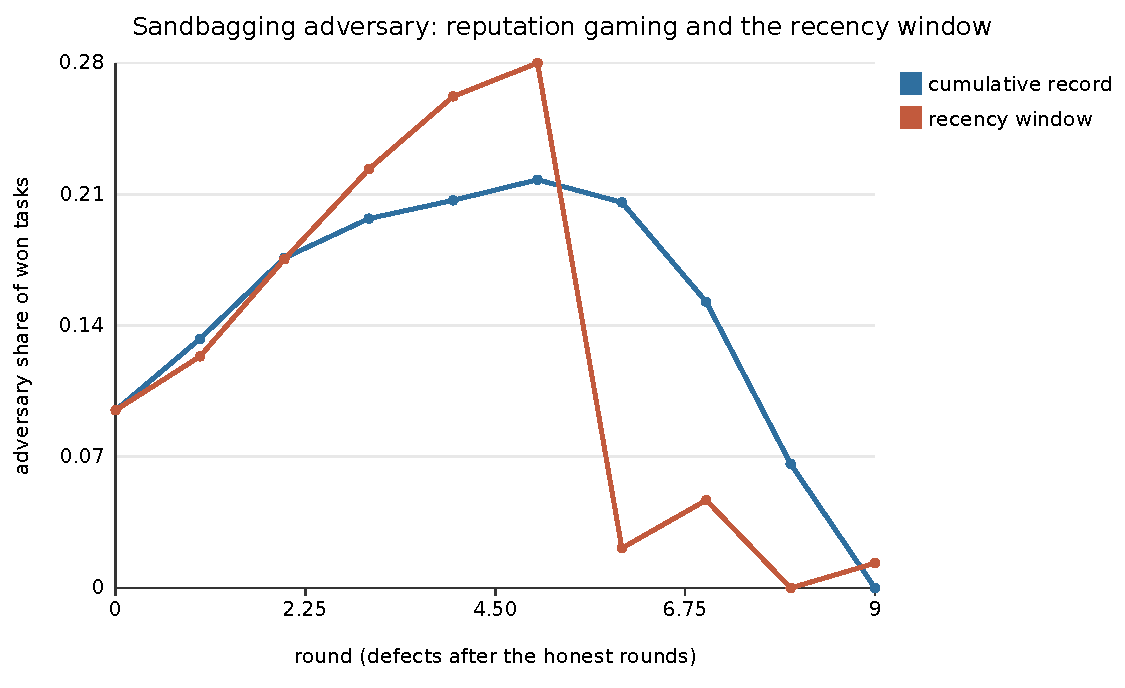
\includegraphics[width=0.80\linewidth]{sandbagging_adversary.pdf}
\caption{The sandbagging adversary builds a clean record over the honest rounds, then defects. Under a cumulative record its win share coasts down over several rounds; a recency-weighted window collapses it the round after defection.}
\label{fig:sandbag}
\end{figure}

\begin{figure}[t]
\centering
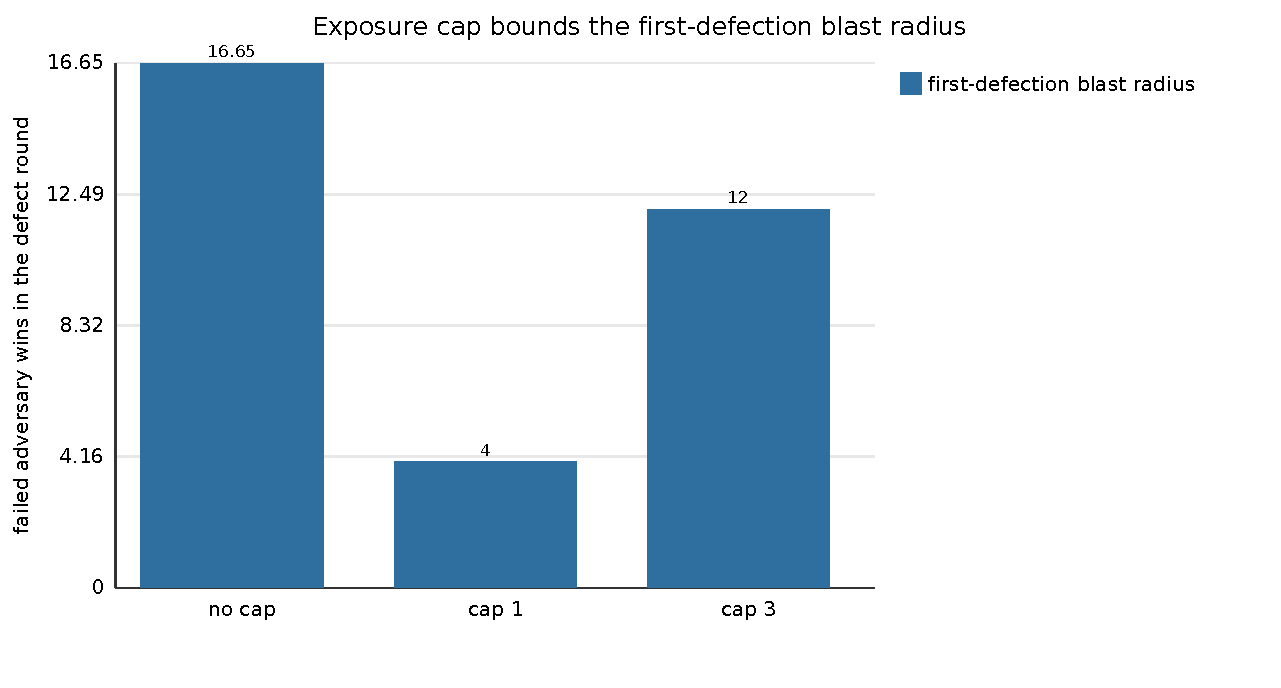
\includegraphics[width=0.80\linewidth]{exposure_cap.pdf}
\caption{Failed adversary wins in the defection round fall from $\approx 17$ with no cap to $\approx 4$ at a cap of one task per agent per round. The cap bounds how much a single newly-defecting agent can sweep before the recency window and the gate react, at a coverage cost.}
\label{fig:exposure}
\end{figure}

\paragraph{Generalisation of the wrapper lift.} To test whether the task-wrapper lift generalises beyond the primary tier, we built a second, structurally independent tier of eight different trap-dense tasks, disjoint from the primary tier, and ran Haiku and Sonnet under the same bare-versus-wrapped design at three agents per cell. Both models solved every task in both conditions (completion $1.00$, lift $0.00$). This is an honest bound rather than a null: the wrapper repairs specific, real failures (on the primary tier the $+0.036$ Haiku lift came from one genuine failure mode), and where the model is already reliable the contract is a no-op with no regression, a safety net rather than a generic booster.

\paragraph{Generalisability across generators.} We re-ran the population-dependent hypotheses under a structurally different \code{latent} family (smooth cosine compatibility, no skill gate). The verdicts hold under both families. The calibration recovery is also robust to how the miscalibration is generated: on a population whose per-agent bias is drawn from the measured MarketBench archetype mixture, the correction still recovers completion by $\approx 0.48$. The full verdicts under both the domains family and the latent family are summarised in Table~\ref{tab:robust}.

\begin{table}[h]
\centering\small
\caption{Verdicts under two structurally different generators.}
\label{tab:robust}
\begin{tabular}{@{}lcc@{}}
\toprule
\textbf{Hypothesis} & \textbf{Domains family} & \textbf{Latent family} \\
\midrule
H2 quality within margin & not supported & not supported \\
H4 safety gate reduces violations & supported & supported \\
H7 self-reports over-predict & supported & supported \\
H8 track record recovers & supported & supported \\
\bottomrule
\end{tabular}
\end{table}

\subsection{Real agents: the two wrappers}
To observe miscalibration rather than just model it, we had real Claude coding agents state their confidence on coding micro-tasks with hidden edge-case tests, then solve them one-shot with no tools. Across a nineteen-task suite over two model families (114 attempts), every attempt passed, at a mean stated confidence of $\approx 0.93$. So both families were underconfident (overconfidence gap $\approx -0.07$), matching the direction MarketBench reports for the Claude models. The sign of the bias depends on the model. That is exactly why the correction reweights by an observable track record: it does not need to know the direction in advance.

To separate model capability from what the wrappers buy, we built a harder expert tier of eight trap-dense tasks and ran three model families (Haiku 4.5, Sonnet 5, Opus 4.8) under two prompts: a bare prompt and a task-wrapped prompt. Over ten Haiku agents per cell, the task wrapper lifts Haiku from $0.950$ (CI $[0.90,0.988]$) to $0.986$ (CI $[0.958,1.00]$), and leaves the already-saturated stronger models unchanged (Figure~\ref{fig:ladder}). The agent wrapper is Binding-Energy routing across this ladder. Over task-wrapped tasks it holds completion at $0.986$ for $\approx 1/47$ of the always-frontier cost; over bare tasks it reaches $0.950$ for $\approx 1/50$ (Figure~\ref{fig:cost}). The two wrappers are complementary: the task wrapper raises the weak model's fidelity, and the agent wrapper turns that into a cost saving. The ladder rests on ten agents per cell with bootstrap CIs; the project on five.

\begin{figure}[t]
\centering
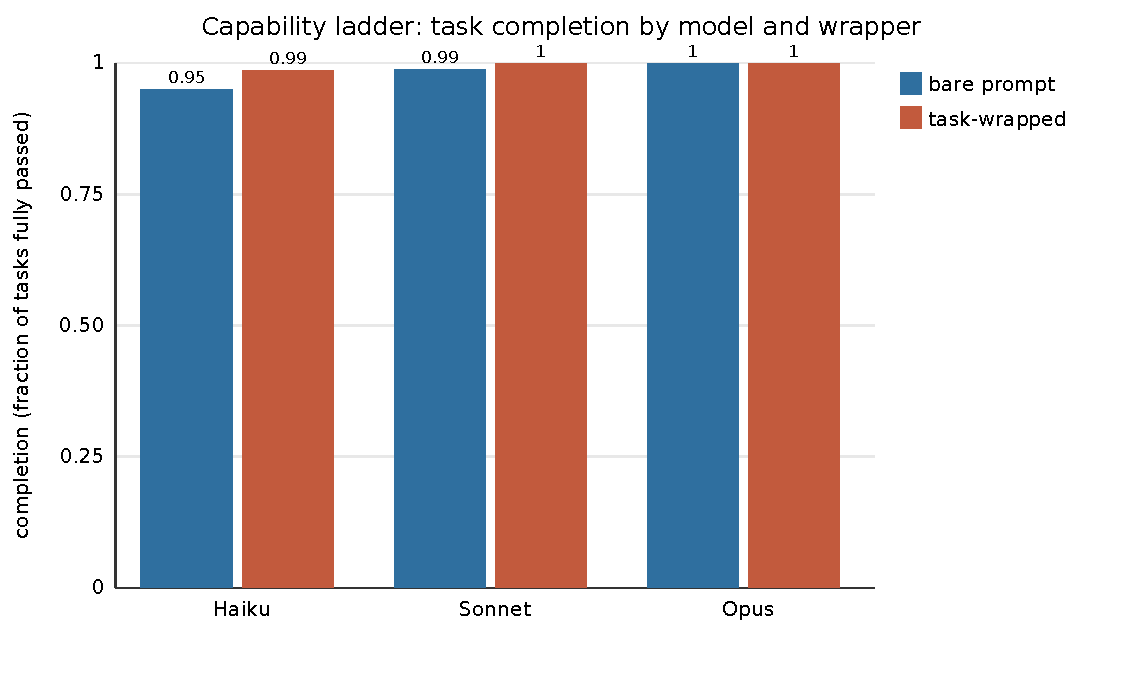
\includegraphics[width=0.86\linewidth]{ladder_completion.pdf}
\caption{The task wrapper (H11) lifts the weakest model to the frontier's completion and leaves the already-saturated models unchanged. Bars are completion; the wrapper helps most where the model is weakest.}
\label{fig:ladder}
\end{figure}

\begin{figure}[t]
\centering
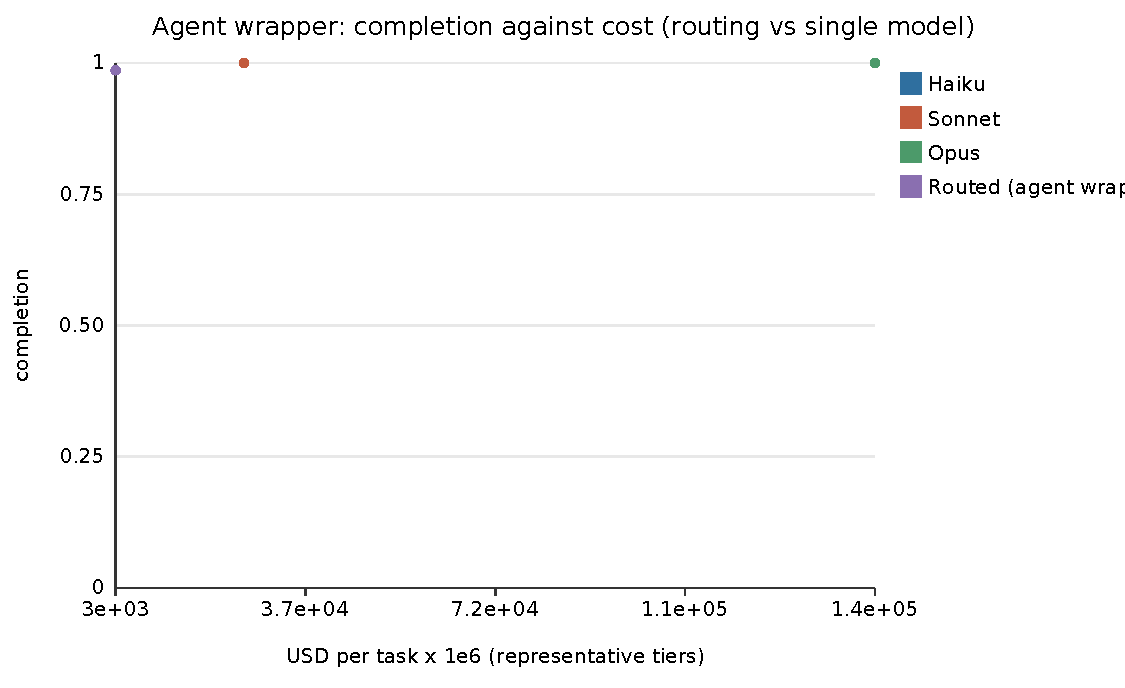
\includegraphics[width=0.86\linewidth]{ladder_cost_fidelity.pdf}
\caption{The agent wrapper (H12). Routing over task-wrapped tasks holds frontier completion at a fraction of the always-frontier cost; over bare tasks it leaves the cheap model's residual gap. Cost is on a representative-tier scale.}
\label{fig:cost}
\end{figure}

To test the wrappers on software that has to be decomposed, rather than on flat tasks, we built \emph{miniquery}: a five-module in-memory query toolkit with a dependency graph and a hidden contract. Each model family built the whole project under the bare and the task-wrapped spec. Under the bare spec every model failed. Each one made a self-consistent but different interface choice, so the modules did not fit together, and completion was zero for all three (Figure~\ref{fig:project}). A calibration signal falls out of the ambiguity: the stronger models correctly lowered their confidence (Sonnet $0.43$, Opus $0.62$), while the weakest stayed overconfident (Haiku $0.89$, on a two-of-five result). The task wrapper is the exact interface contract, and with it every model delivered a fully conforming project (completion $1.0$). The agent wrapper then assembles the cross-model project for $\approx 1/39$ of the always-frontier cost, whereas the bare assembly fails at any price, because no model produced a conforming \code{render} without the contract.

\begin{figure}[t]
\centering
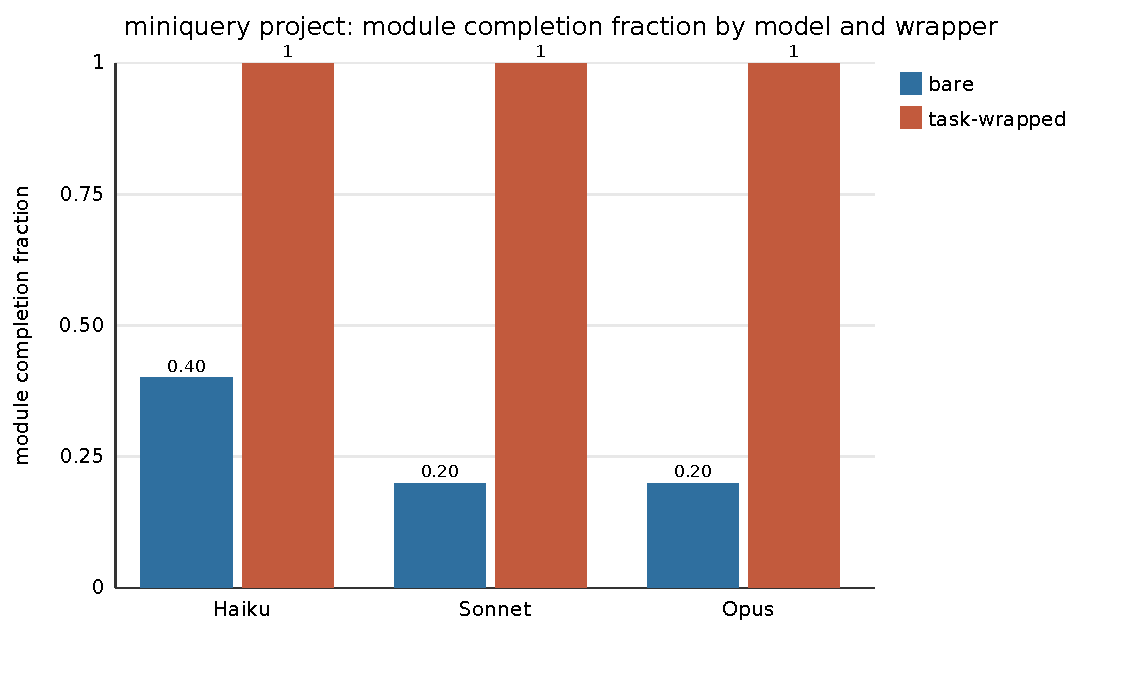
\includegraphics[width=0.86\linewidth]{project_modules.pdf}
\caption{The dependency-graph project. Under a loose spec every model, including the frontier one, ships a divergent interface and no working project; the interface contract makes all three deliver a conforming five-module project. Capability does not rescue integration; the contract does.}
\label{fig:project}
\end{figure}

\section{Discussion}

The runs support the scaling and expressiveness claims, and the repositioning around calibration turns the earlier soft spots into results. The quality claim H2 does not hold against a fair optimum, and we report that as it stands. On scaling: once we measure the bottleneck as peak per-node load and let each agent observe only a bounded sample of tasks, CTA's peak load is flat in the population size, while the central scheduler grows with $N\times M$. A log-log fit recovers the two growth orders cleanly. On quality: against the fair full-information optimum (\code{central\_best}, agent reuse allowed), CTA reaches $\approx 94\%$ of the optimum and is level with pull-based. Breaking the gap down, about three quarters of it is quality the cost-aware bid trades for lower latency by design, and only about a quarter is the residual from ranking on a noisy track record. So CTA is not failing to find quality; it is optimising quality per unit cost.

The central result is about the assumption self-selection rests on. When the compatibility bid is the agent's own self-report and competence varies, the raw self-report auction is competence-blind: completion falls to $\approx 0.37$, while the winners over-predict their own quality by $\approx 0.20$ (H7). The fix is cheap and needs no privileged information. Discounting each self-report by the observable track record raises completion to $\approx 0.76$, a recovery of $\approx 0.39$ that stays highly significant after multiple-comparison correction (H8). We also argue the H6 comparison against a full-information optimum is the wrong test for a deployment, because that optimum cannot exist in production. H9 replaces it with the bounded central scheduler a deployment would actually run. CTA is level with that scheduler when its table is fresh, and pulls decisively ahead as the table goes stale, because a decentralised agent never pays the synchronisation lag a central table does.

On external validity, the miscalibration is not just a synthetic knob. A fleet parameterised from MarketBench reproduces the effect, and a live pilot with real Claude agents confirms on real data that a coding agent's self-reports are miscalibrated. On solvable in-distribution tasks the direction is underconfidence, so a naive auction would under-select capable agents rather than over-select bad ones. The harder tier did not flip that sign, so the overconfident failure region is out-of-distribution here; reaching it would need tasks beyond a model's competence, or a model family that is overconfident in-distribution. This loop is a \emph{harness} in the sense recent work gives the term \citep{weng2026harness}: the software around a base model that decides how it plans, what it remembers, and how its work is judged. That work's diagnosis is that a self-improving loop is only as good as the signal it optimises, and the evaluator is the weak link. CTA's track-record correction turns an unreliable self-report into a trustworthy allocation signal, and H13 makes the self-improvement concrete. We therefore claim CTA as the calibration-robust signal layer of such a harness, not as a full self-improving system.

The scaling result has a direct commercial reading. Turn the pair-evaluation count into money at representative prices. A central scheduler that scores every agent-task pair pays a bill that grows as $N\times M$. A decentralised fleet caps each agent at a bounded sample, so the busiest node's bill is flat and the total grows only linearly. At the standard tier the central cost per allocation round rises from $\approx\$14$ at a hundred agents to $\approx\$144{,}000$ at ten thousand, whereas the decentralised total is $\approx\$576$ and no single node pays more than $\approx\$0.06$: a $\approx 250\times$ saving at the top of the range. That shape, a quadratic central bill against a flat per-node decentralised one, is a property of the coordination structure, not of the prices.

\paragraph{Where this research stands.} Eleven pre-registered hypotheses on synthetic populations are evaluated at full protocol scale, nine supported and two reported as honest negatives. Two further hypotheses (the task-wrapper lift and the calibrated-routing cost-efficiency) are added on real Claude agents and supported with bootstrap confidence intervals: the ladder rests on about ten agents per cell and the project on five. It is a mechanism study with real-agent confirmation, not a benchmarked production system, and every claim is marked against that boundary. The natural next step is a head-to-head against a named router on a shared, established benchmark.

\section{Building the wrappers}

\paragraph{The task wrapper.} A task wrapper is an explicit interface contract. It has a name, a signature, a one-line description, a set of named acceptance criteria, a few worked examples, and a short self-check the agent runs before it commits. The orchestrator owns and builds it, which keeps it stable across a mixed fleet. You can build it from a machine-checkable spec, from examples, from a natural-language description via a cheap wrapping model, or from downstream integration failures added as new acceptance clauses. The design rule is simple: the acceptance criteria should name the properties a hidden test would check. The lift comes from surfacing the unstated edge cases that separate a competent-looking answer from a correct one.

\paragraph{The agent wrapper.} The agent wrapper turns a fleet of models into one calibrated router. Each model has a price tier; the fleet holds the models cheapest first, plus a per-task reliability table. Routing is one rule. Each model reports a self-assessed confidence. The bid is discounted by that model's reliability on this kind of task. The task then goes to the cheapest model whose corrected bid clears the barrier, or, if none clears it, escalates to the highest corrected bid. Reliability is updated after each outcome by a moving average, so the router learns the fleet from the first real results instead of assuming a fixed capability. That is the difference from a static-capability router.

\paragraph{The loop.} The two wrappers are not a single call but a loop, and the loop is where the results compound. The track record sharpens, so more tasks safely drop to cheaper models. The task contracts sharpen from integration failures, so weak models grow more reliable on exactly the tasks that used to break them. Calibration robustness and cost efficiency are properties of this loop, not of any one allocation.

\section{Outlook and conclusion}

The dominant pattern today is a single large model called once per task, sometimes fronted by a router that picks a model by static capability. That pattern pays frontier-token prices everywhere, and, as the project experiment shows, it cannot split a task across independent workers without an interface contract. The alternative this work supports is a swarm of microagents: small, cheap, specialised workers, each inside a tight harness, coordinated by calibrated self-selection. The claim to a breakthrough rests on combining three things usually pursued separately. First, a decentralised substrate that removes the coordinator bottleneck. Second, a routing rule that corrects the self-report by an observable track record and screens the winner for safety. Third, a task wrapper: the contract that makes a swarm's output fit together. If the real-agent results hold at scale, we can grow agent systems by the count of cheap microagents rather than the size of one model, a different and far cheaper axis of growth.

In summary, CTA is a decentralised, biomimetic framework in which tasks advertise contracts and agents self-select by a calibrated, reliability-weighted, gated bid. It holds the busiest node's coordination load flat as the fleet grows to ten thousand agents. It names and fixes the failure mode of self-selection, miscalibration, recovering the completion it costs with a track-record correction that uses no privileged information. And on real Claude agents, the two wrappers turn the mechanism into a cost result, holding frontier-level completion at roughly one fortieth of the always-frontier cost. The practical thesis is that a swarm of cheap, wrapped microagents coordinated by calibrated self-selection can match a single expensive model at a fraction of its cost, and that is the direction this work opens.

\bibliographystyle{plainnat}
\bibliography{refs}

\end{document}
